%% LaTeX .tex
%% Template para a 2ª Escola Brasileira de Dinâmica de Rotores
%% EBDR 2026
%% 17-18 de setembro de 2026, Uberlândia

\documentclass[10pt,fleqn,a4paper,twoside]{article}
\usepackage{EBDR2026}
\def\shortauthor{P. Autor, S. Autor e T. Autor (atualize este cabeçalho conforme necessário)}
\def\shorttitle{Título Curto do Artigo (Iniciais Maiúsculas, garantir que caiba em uma linha)}

\begin{document}
\fphead
\hspace*{-2.5mm}\begin{tabular}{||p{\textwidth}}
\begin{center}
\vspace{-4mm}
\title{INSTRUÇÕES PARA FORMATAÇÃO DE ARTIGOS (VERSÕES PRELIMINAR E FINAL) DA EBDR 2026} %(XXXX é o número do manuscrito. Ele estará disponível após a submissão do resumo expandido e deve ser incluído na submissão do artigo final.)
\end{center}
\authors{Nome do Primeiro Autor} \\
\authors{Nome do Segundo Autor} \\
\institution{Instituição e endereço para o primeiro e segundo autores - se forem os mesmos} \\
\institution{e-mails} \\
\\
\authors{Nome do Terceiro Autor} \\
\institution{Instituição e endereço para o terceiro autor} \\ %(Se todos os autores forem da mesma instituição, "Instituição e endereço" deve ser informado apenas uma vez.)
\institution{e-mail} \\
\\
\authors{Mesmo formato para outros autores, se houver} \\
\\
\abstract{\textbf{Resumo.} O resumo deve descrever os objetivos, a metodologia e as principais conclusões do artigo em aproximadamente 200 palavras. Não deve conter fórmulas nem referências bibliográficas.}\\
\\
\keywords{\textbf{Palavras-chave:} palavra-chave 1, palavra-chave 2, palavra-chave 3\dots{} (até 5 palavras-chave)}\\
\end{tabular}

\section{INTRODUÇÃO}

O objetivo destas instruções é servir como guia para a formatação de artigos a serem publicados nos Anais da 2ª Escola Brasileira de Dinâmica de Rotores (EBDR 2026).

Os Anais da EBDR 2026 serão publicados em formato Adobe\texttrademark\space PDF.

Os artigos {\bf DEVEM} ser formatados rigorosamente de acordo com estas instruções. O presente arquivo pode ser utilizado como modelo para usuários de \LaTeX\space. Também pode ser utilizado como guia de formatação para usuários de outros softwares de processamento de texto.

Recomenda-se que o artigo tenha no máximo {\bf 4} páginas, incluindo tabelas e figuras.

\section{FORMATAÇÃO DO TEXTO}

Os manuscritos devem ser escritos em português, digitados em páginas no formato A4, utilizando fonte Times New Roman, tamanho 10, exceto para o título, afiliação dos autores, resumo e palavras-chave, para os quais instruções específicas de formatação são indicadas acima. Deve-se utilizar espaçamento simples entre linhas em todo o texto.

O bloco de texto que contém o título, os nomes dos autores e suas afiliações, o resumo e as palavras-chave deve ser recuado em 0,1 cm a partir da margem esquerda e marcado por uma linha preta vertical à esquerda com espessura de 2 1/4 pt.

A primeira página deve ter margem superior de 3 cm e as demais margens (esquerda, direita e inferior) devem ter 2 cm. Todas as demais páginas devem ter todas as margens iguais a 2 cm.

AS PÁGINAS {\bf NÃO DEVEM} SER NUMERADAS

O corpo do texto deve ser justificado. A primeira linha de cada parágrafo deve ter recuo de 0,5 cm. Informações suficientes devem ser fornecidas diretamente no texto ou por meio de referências a trabalhos amplamente disponíveis na literatura. Notas de rodapé devem ser evitadas.

Todos os símbolos e notações devem ser definidos no texto. As grandezas físicas devem ser expressas no Sistema Internacional de Unidades (SI). Símbolos matemáticos que aparecem no texto devem ser escritos em itálico.

As referências bibliográficas devem ser citadas no texto pelo sobrenome do(s) autor(es) e ano de publicação, de acordo com os seguintes exemplos: ``Em um trabalho recente~\citep{BandarraFilho2011}\dots'' ou ``Recentemente, \citet{BandarraFilho2011}\dots''. No caso de três ou mais autores, deve-se utilizar a forma ``\citep{CavaliniJunior2015}''. Duas ou mais referências com os mesmos autores e ano de publicação devem ser diferenciadas acrescentando ``a'', ``b'', etc., ao ano. Por exemplo: ``Nos trabalhos~\citep{Santos2013a} e \citep{Santos2013b}\dots''.

Referências aceitáveis incluem artigos de periódicos~\citep{MLA04}, artigos numerados, dissertações e teses~\citep{CavaliniJunior2013,coelho2017}, anais de congressos publicados, preprints de conferências, livros~\citep{McConnell.Varoto.2008} e artigos submetidos (desde que o periódico seja identificado).

As referências devem ser listadas ao final do artigo de acordo com as instruções fornecidas na Seção 4.

\subsection{Títulos de seções e subseções}

Os títulos de seções e subseções devem ser alinhados à esquerda, digitados em fonte Times New Roman, tamanho 10, em negrito. Devem ser numerados utilizando algarismos arábicos separados por pontos. Não devem ser utilizados mais do que 3 níveis de subseções. Deve-se incluir uma linha em branco acima e abaixo de cada título de seção/subseção.

\subsection{Equações matemáticas}

As equações matemáticas devem ser recuadas em 0,5 cm a partir da margem esquerda. Devem ser digitadas em fonte Times New Roman, itálico, tamanho 10 pt. Algarismos arábicos devem ser utilizados para numerar as equações, entre parênteses e alinhados à direita, conforme mostrado nos exemplos abaixo. As equações devem ser referenciadas como ``Eq.~(\ref{eq1})'' no meio de uma frase ou como ``Equação~(\ref{eq1})'' no início de uma frase. Quantidades matriciais e vetoriais podem ser indicadas por colchetes e chaves, como na Eq.~(\ref{eq1}), ou em negrito, como na Eq.~(\ref{eq2}). Os símbolos utilizados nas equações devem ser definidos imediatamente antes ou após sua primeira aparição.

Deve-se incluir uma linha em branco acima e abaixo de cada equação.
\begin{equation}
[M]\{\ddot{x}\}+[C]\{\dot{x}(t)\}+[K]\{x(t)\}={f(t)} 
\label{eq1}
\end{equation}
\begin{equation}
\mathbf{M\ddot{x}}(t)+\mathbf{C\dot{x}}(t)+\mathbf{Kx}(t)=\mathbf{f}(t) 
\label{eq2}
\end{equation}

\subsection{Figuras e Tabelas}

Figuras e tabelas devem ser posicionadas no texto o mais próximo possível do ponto onde são mencionadas pela primeira vez e devem ser numeradas consecutivamente em algarismos arábicos. As figuras devem ser referenciadas como ``Fig.~\ref{fig1}'' no meio de uma frase ou como ``Figura~\ref{fig1}'' no início de uma frase. As figuras, bem como suas legendas, devem ser centralizadas na direção horizontal. As legendas das figuras não devem ultrapassar 3 linhas.

A legenda dos símbolos dos dados, bem como os rótulos de cada curva, devem ser incluídos na figura. Os textos devem ter tamanho suficiente para facilitar a leitura. Todas as unidades devem ser expressas no Sistema Internacional (SI).

Deve-se deixar uma linha em branco antes e depois de cada figura.
\begin{figure}[h!]
\centering
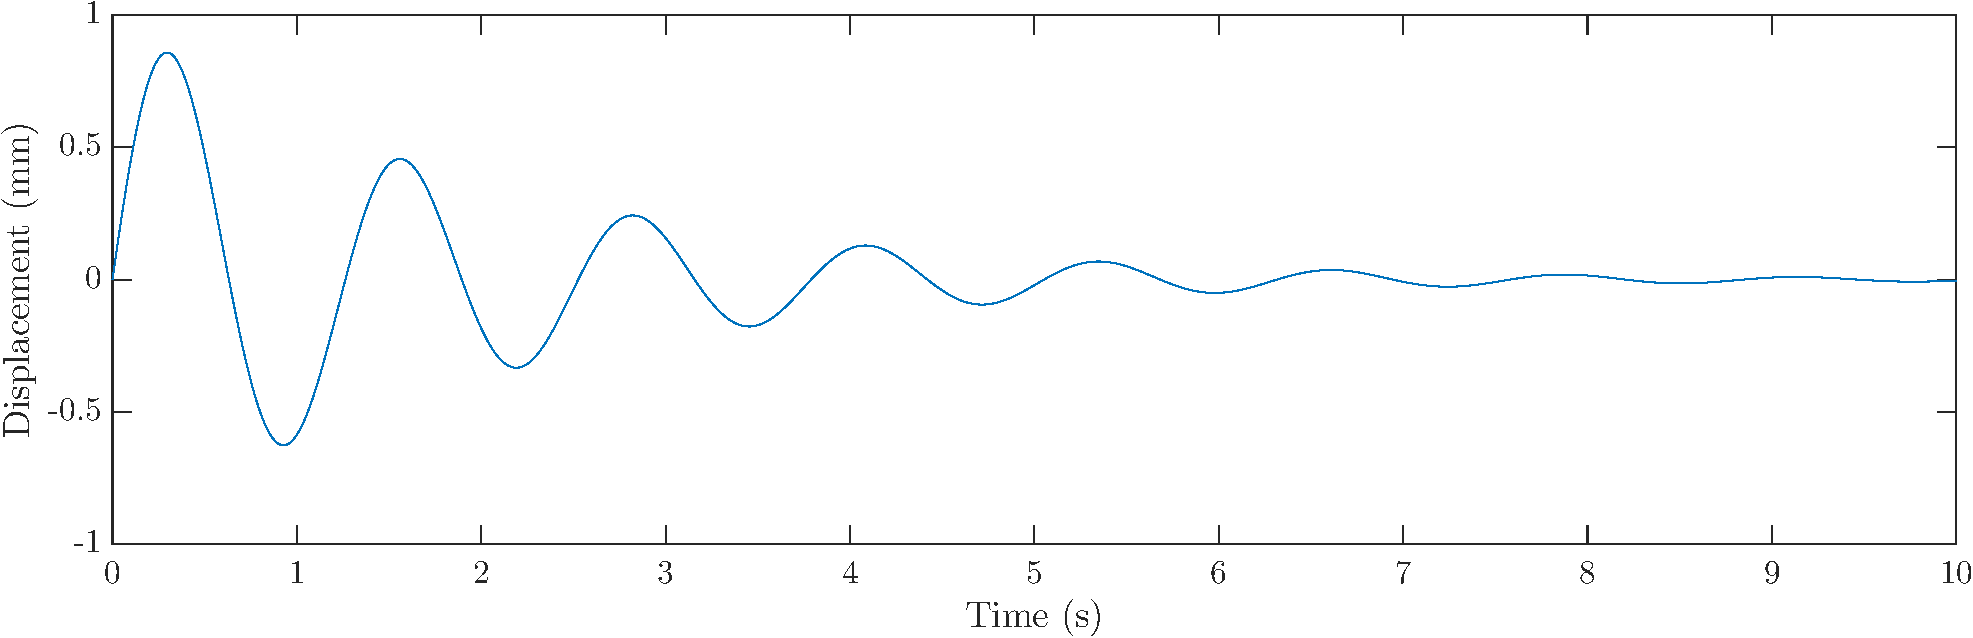
\includegraphics[width=150mm]{Figures/figure1.pdf}
\caption{Resposta do sistema quando submetido a uma força impulsiva.}
\label{fig1}
\end{figure}

Figuras coloridas e fotografias de alta qualidade podem ser incluídas no artigo. Para reduzir o tamanho do arquivo e preservar a resolução gráfica, as figuras devem ser salvas em formato GIF (figuras com menos de 16 cores) ou JPEG (para maior densidade de cores) antes de serem inseridas no manuscrito.

As tabelas devem ser referenciadas como ``Tab.~\ref{tab1}'' no meio de uma frase ou como ``Tabela~\ref{tab1}'' no início de uma frase. As tabelas, bem como seus títulos, devem ser centralizadas na direção horizontal. Os títulos das tabelas não devem ultrapassar 3 linhas. O estilo e tamanho da fonte utilizados nas tabelas devem ser semelhantes aos utilizados no corpo do texto. As unidades devem ser expressas no Sistema Internacional (SI). Explicações, se houver, devem ser apresentadas no rodapé das tabelas, e não dentro delas.

Deve-se deixar uma linha em branco antes e depois de cada tabela.

O estilo das bordas das tabelas é livre. Um exemplo é apresentado na Tab.~\ref{tab1}.
\begin{table}[!h]
\centering
\caption{Resultados experimentais das propriedades de flexão dos compósitos CFRC-4HS e CFRC-TWILL. \protect\\Relação vão/profundidade = 35:1. Resultados médios de 7 espécimes.}
\begin{tabular}{|c|c|c|}
\hline
Propriedades do Compósito & CFRC-TWILL & CFRC-4HS\\
\hline
Resistência à flexão (MPa)$^{(1)}$ & 209$\pm$ 10 & 180 $\pm$  15\\
\hline
Módulo de flexão (GPa)$^{(1)}$ & 57.0 $\pm$ 2.8 & 18.0 $\pm$  1.3\\
\hline
Deflexão no meio do vão na tensão de falha (mm) & 2.15 $\pm$  1.90 & 6.40 $\pm$  0.25\\
\hline
\end{tabular}
\\
\begin{tabular}{p{11cm}ll}
$^{(1)}$ medido a 25$^{o}$C & &
\end{tabular}
\label{tab1}
\end{table}

\section{AGRADECIMENTOS}
Esta seção é opcional e deve ser posicionada antes da lista de referências.

\section{REFERÊNCIAS} 

A lista de referências deve ser apresentada como uma nova seção, localizada ao final do artigo. A primeira linha de cada referência deve ser alinhada à esquerda. Todas as demais linhas devem ter recuo de 0,5 cm a partir da margem esquerda. Todas as referências incluídas na lista devem ter sido citadas no texto.

As referências devem ser listadas em ordem alfabética, de acordo com o sobrenome do primeiro autor. Veja os exemplos a seguir:

\bibliographystyle{EBDR2026}
\renewcommand{\refname}{}
\bibliography{bibfile}

\section{TERMO DE RESPONSABILIDADE}

O seguinte texto, devidamente adaptado ao número de autores, deve ser incluído na última seção do artigo:

O(s) autor(es) é (são) o(s) único(s) responsável(is) pelo conteúdo publicado neste artigo.

\end{document}
